\chapter{Results and Discussions}
In this section we will compare the results our smoothing algorithm with other leplacian smoothing algorithms for 2D and 3D meshes. We will discuss the results based on aspect ratio distribution and min angle criteria, though aspect ratio and min angle are related for triangular and tetrahedral meshes.

Figure \ref{fig:points_1000} shows our smoothing algorithm with and without flipping for smart laplacian and our aspect ratio based smoothing. Square contains approximately  100 points and original figure shows the delaunay points. It's a bad triangulation to start with but effectiveness of our algorithm can be seen from comparing laplacian with flipping and our algorithm with flipping. Laplacian is very efficient for 2D triangular meshes as it can be seen in Figure \ref{fig:points_1000}(c). Our algorithm improves upon the smart laplacian and distributes the area and min angles much  better than smart laplacian shown in Figure \ref{fig:points_1000}(e).

\begin{figure}[h]
    \centering
    \begin{subfigure}[h]{1.0\textwidth}
        \centering
        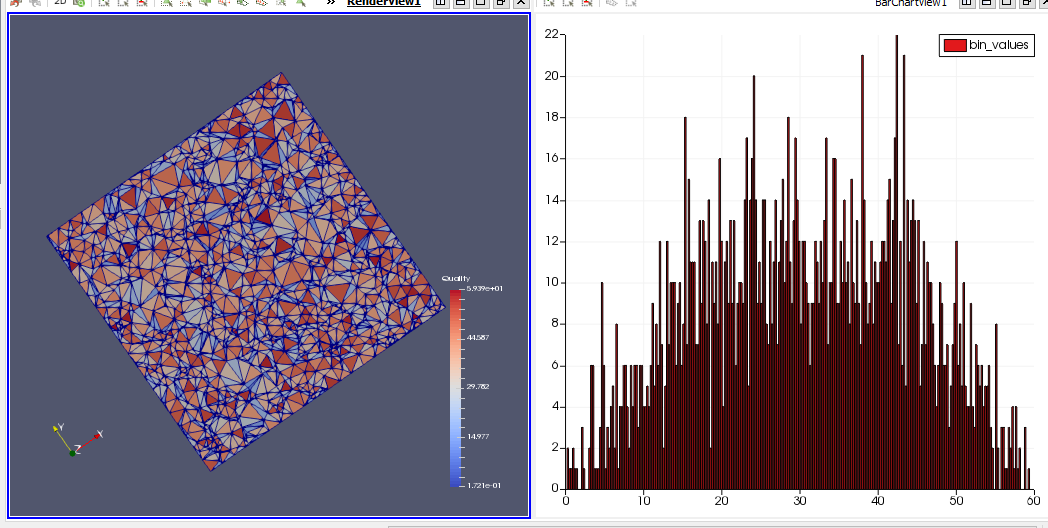
\includegraphics[width=\textwidth]{images/original_1000.png}
        \caption{Original}
    \end{subfigure}
    \vspace{0.5 cm}

    \begin{subfigure}[h]{1.0\textwidth}
        \centering
        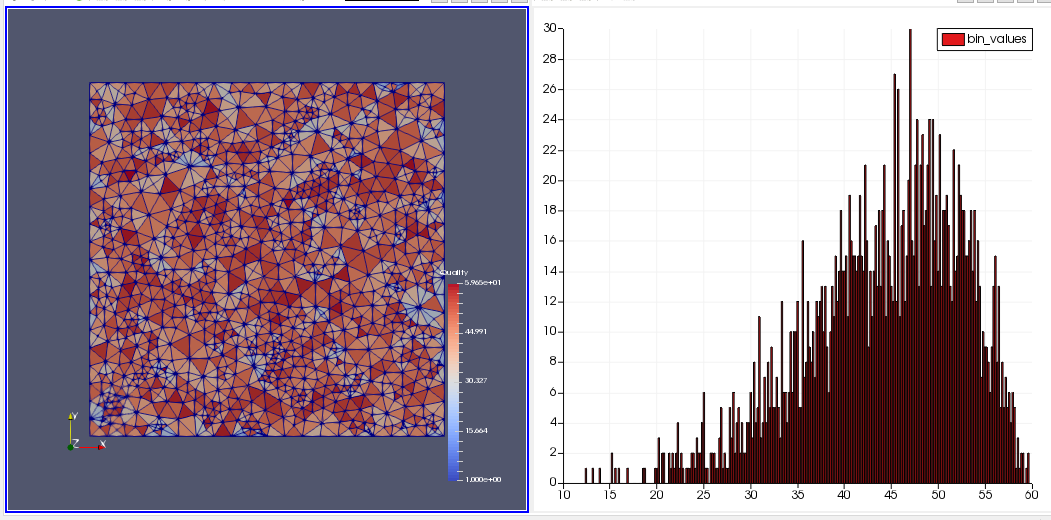
\includegraphics[width=\textwidth]{images/laplacian_no_flips_1000.png}
        \caption{Smart Laplacian without flips}
    \end{subfigure}
    \vspace{0.5 cm}
 
    \begin{subfigure}[h]{1.0\textwidth}
        \centering
        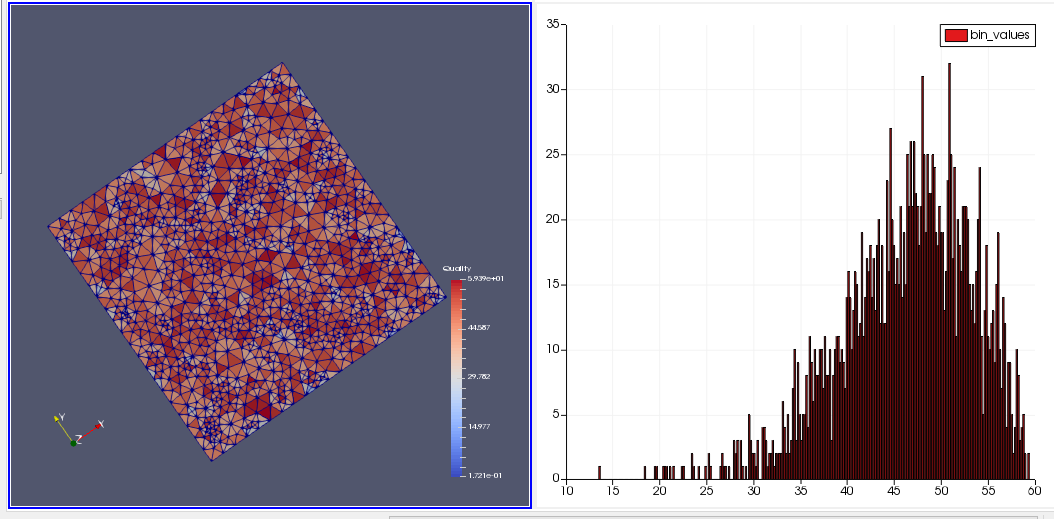
\includegraphics[width=\textwidth]{images/laplacian_1000.png}
        \caption{Smart Laplacian with flips}
    \end{subfigure}
	\vspace{0.5 cm}
\end{figure}

\begin{figure}[h]
	\ContinuedFloat
    \centering
   	\begin{subfigure}[h]{1.0\textwidth}
        \centering
        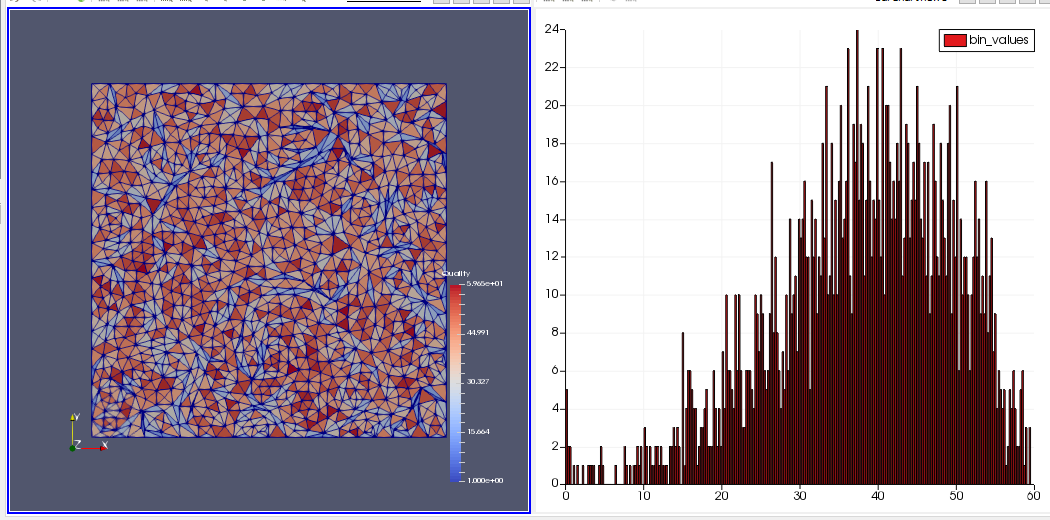
\includegraphics[width=\textwidth]{images/aspect_ratio_no_flips_1000.png}
        \caption{Aspect Ratio Based without flips}
    \end{subfigure}
	\vspace{0.5 cm}
   
    \begin{subfigure}[h]{1.0\textwidth}
        \centering
        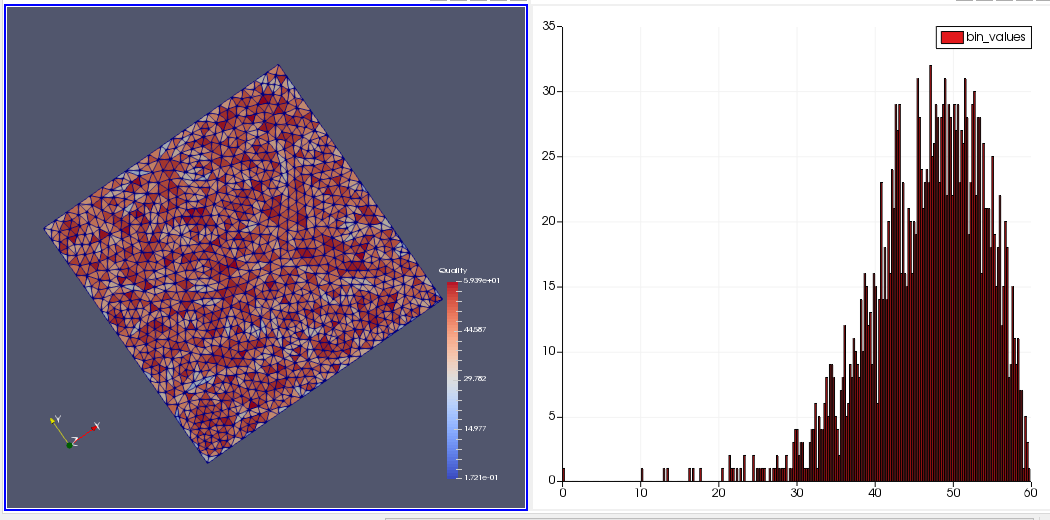
\includegraphics[width=\textwidth]{images/aspect_ratio_1000.png}
        \caption{Aspect Ratio Based with flips}    
    \end{subfigure}	  	
    \caption{Delaunay mesh of square having 1000 vertices}
    \label{fig:points_1000}
\end{figure}

\section{Implementation Details}
We implemented incremental delaunay triangulation for 2D and 3D using flips in C++. For 2D, we used half edge data structure and it can robustly handle upto million points.
For 3D, we used tetrahedron based data structure based on Tetgen \cite{tetgen}. For robustness, we used Jonathan Schewchuck's code for robust predicates which is free for academic purposes. We used 2.2 GHz machine with 8 GB RAM to generate our results. We used extensively Paraview based on VTK geometric library for generating  snapshots and graphs for distribution of aspect ratios and min angles.